\documentclass[12pt]{article}

\usepackage{fullpage}
\usepackage{multicol,multirow}
\usepackage{tabularx}
\usepackage{graphicx}
\usepackage{ulem}
\usepackage[utf8]{inputenc}
\usepackage[russian]{babel}


\begin{document}

\section*{Лабораторная работа №\,1 по курсу дискрeтного анализа: сортировка за линейное время}

Выполнил студент МАИ группы М8О-201Б \textit{Ефимов Александр}.

\subsection*{Постановка задачи}


Необходимо создать программную библиотеку, реализующую указанную структуру данных, на основе которой разработать программу-словарь. В словаре каждому ключу, представляющему из себя регистронезависимую последовательность букв английского алфавита длиной не более 256 символов, поставлен в соответствие некоторый номер, от 0 до 264 - 1. Разным словам может быть поставлен в соответствие один и тот же номер.

Программа должна обрабатывать строки входного файла до его окончания. Каждая строка может иметь следующий формат:\\
\textbf{+ word 34} — добавить слово «word» с номером 34 в словарь. Программа должна вывести строку «OK», если операция прошла успешно, «Exist», если слово уже находится в словаре.\\
\textbf{- word} — удалить слово «word» из словаря. Программа должна вывести «OK», если слово существовало и было удалено, «NoSuchWord», если слово в словаре не было найдено.\\
\textbf{- word} — найти в словаре слово «word». Программа должна вывести «OK: 34», если слово было найдено; число, которое следует за «OK:» — номер, присвоенный слову при добавлении. В случае, если слово в словаре не было обнаружено, нужно вывести строку «NoSuchWord».\\
\textbf{! Save /path/to/file} — сохранить словарь в бинарном компактном представлении на диск в файл, указанный парамером команды. В случае успеха, программа должна вывести «OK», в случае неудачи выполнения операции, программа должна вывести описание ошибки (см. ниже).\\
\textbf{! Load /path/to/file} — загрузить словарь из файла. Предполагается, что файл был ранее подготовлен при помощи команды Save. В случае успеха, программа должна вывести строку «OK», а загруженный словарь должен заменить текущий (с которым происходит работа); в случае неуспеха, должна быть выведена диагностика, а рабочий словарь должен остаться без изменений. Кроме системных ошибок, программа должна корректно обрабатывать случаи несовпадения формата указанного файла и представления данных словаря во внешнем файле.

Для всех операций, в случае возникновения системной ошибки (нехватка памяти, отсутсвие прав записи и т.п.), программа должна вывести строку, начинающуюся с «ERROR:» и описывающую на английском языке возникшую ошибку.\\
  
 \ Вариант 5: \textit{B-Tree}

\subsection*{Метод решения}


В соответствии с ограничениями требуется реализация следующих функций
\begin{enumerate}
\item Поиск по ключу
\item Добавление и удаление по ключу
\item Сохранение в файл и загрузка из него
\end{enumerate}
Для удобства работы с ключами, представленных строками, используется функция библиотеки \textbf{<cstring>} \textit{strcmp} для сравнения лексикографического порядка \\

Поиск по ключу является простой операцией сравнения ключей (или в данном случае лекискографического порядка строк) и вывода успеха, если ключ найден, и неуспеха, если в листе не найден искомый ключ.

В связи с характеристикой B-Tree, вставка ключа должна происходить за один обход. Это достижимо за счет разбиения полных узлов на 2 равных и перенесения ключа в родителя. Разбиение происходит до входа в узел, что гарантирует наличие места для ключа. Соответственно, операция вставки разбивается еще на две функции \--- разбиения и самой вставки.

Операция удаления является самой сложной, требуя покрытия шести возможных случаев:
\begin{enumerate}
\item Удаление ключа из листа;\\

Удаление ключа из внутреннего узла, при этом
\item Взятие ключа предшествующего ключа (т.е. самого правого ключа из левого поддерева) если количество ключей не меньше $T$, замена им удаляемого ключа и последующее рекурсивное удаление взятого ключа;
\item Взятие ключа последующего ключа если количество ключей не меньше $T$, замена им удаляемого ключа и последующее рекурсивное удаление взятого ключа;
\item Если количество ключей в обоих деревьях меньше $T$, слияние двух обоих узлов в один с внесением в него удаляемого ключа. Ключ рекурсивно удаляется в новом узле.\\

Если при поиске в ребенке текущего узла количество ключей меньше $T$, то
\item Если рядом с предшествующий или последющий ребенку брат имеет $T$ ключей, то совершить правый или левый поворот соответственно
\item Иначе слиять одного из братов с ребенком и добавить к полученному узлу ключ из родителя, указывающий на них
\end{enumerate}

Операции ввода и вывода всего лишь требуют записи и считывания данных в одной и той же последовательности, что легко достигается рекурсией.

\subsection*{Описание программы}

\begin{enumerate}
\item \textbf{b-tree.h и b-tree.cpp}
	\begin{itemize}
	Описывает классы TBTree для дерева и TBTreeNode для узлов
		\item Оба класса описывают методы поиска, добавления, удаления, сохранения и загрузки (\textit{Search}, \textit{Insert}, \textit{Delete}, \textit{Save} и \textit{Load} соответственно);
		\item TBTreeNode отдельно содержит методы разбиения и слияния узлов (\textit{Split} и \textit{Merge}, \textit{PrematureMerge} для слияние перед входом в ребека);
		\item Разбение на два класса помогает рассматривать отдельно корень.
	\end{itemize}
\item \textbf{menu.cpp}
Простое меню, которое принимает ввод и сопоставляет ему необходимые функции. 
\end{enumerate}

\subsection*{Дневник отладки}

\begin{center}
 \begin{tabular}{| c |p{4cm}|p{5cm}|p{4cm}|} 
 \hline
 Номер & Ошибка & Обнаруженная причина &  Исправление \\
 \hline\hline
 1 & Ошибка компиляции & Не обнаружен \textit{Makefile} & Добавить \textit{Makefile}  \\ 
 \hline
 2 & Ошибка выполнения & После удаления последнего ключа корнем мог стать невыделенный ребенок \textit{} & Добавить проверку \textit{leaf} \\
 \hline
 3 & Ошибка выполнения & При закрытии файла Valgrind выдает предупреждение использования неинициализированных байтов & На момент написания отчета \--- не известно \\
 \hline
\end{tabular}
\end{center}

\subsection*{Тест производительности}

\begin{figure}[htp]

\centering
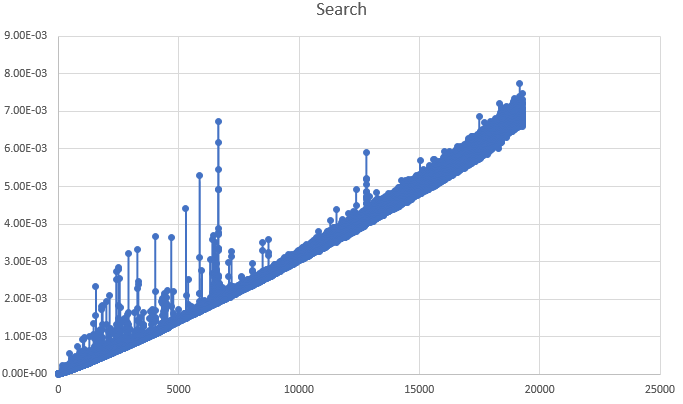
\includegraphics[width=.7\textwidth]{pics/Search.PNG}\hfill
\caption{Поиск}
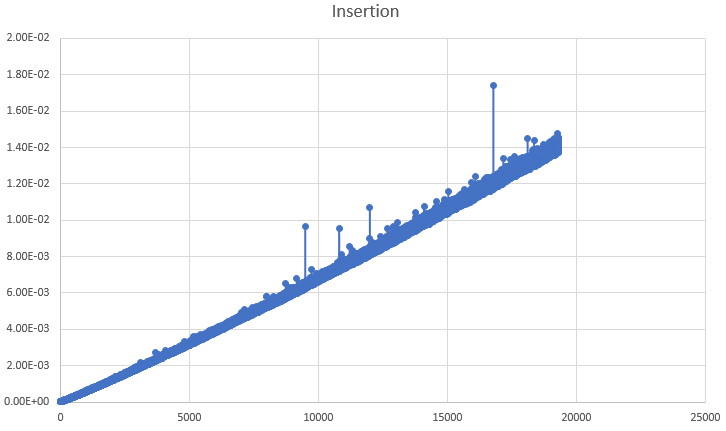
\includegraphics[width=.7\textwidth]{pics/Insertion.PNG}\hfill
\caption{Вставка}
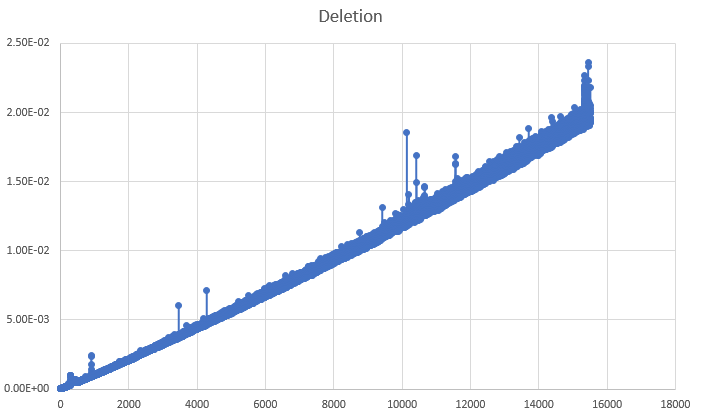
\includegraphics[width=.7\textwidth]{pics/Deletion.PNG}
\caption{Удаление}
\label{fig:figure3}

\end{figure}

На рисунках 1-3 показаны время выполнения каждой из трех операций: поиск, вставка, удаление.\\
Несмотря на сложность худшую сложность $O(t*log(tn))$, операции выполнились за линейное время, что говорит о возможной плохой оптимизации.

\linebreak

\subsection*{Недочёты}

По своим особенностям, b-tree не получает никаких преимуществ, если он работает в памяти. Он создан для уменьшения загрузки страниц когда он записан на диске. При построении дерева в памяти следует выбрать другие структуры, такие как AVL-дерево, или выбрать наимньший возомжный порядок b-tree (т.е. три).

\subsection*{Выводы}

Когда он сохранен на диске, B-Tree позволяет уменьшить количество считываний с него за счет размещения каждого узла на свои страницы (т.е если максимальный порядок равен размеру одной страницы, то весь узел будет размещен на одной странице, что позволяет подгрузить его за один оборот).

\end{document}
